\documentclass[11pt,preprint, authoryear]{elsarticle}

\usepackage{lmodern}
%%%% My spacing
\usepackage{setspace}
\setstretch{1.2}
\DeclareMathSizes{12}{14}{10}{10}

% Wrap around which gives all figures included the [H] command, or places it "here". This can be tedious to code in Rmarkdown.
\usepackage{float}
\let\origfigure\figure
\let\endorigfigure\endfigure
\renewenvironment{figure}[1][2] {
    \expandafter\origfigure\expandafter[H]
} {
    \endorigfigure
}

\let\origtable\table
\let\endorigtable\endtable
\renewenvironment{table}[1][2] {
    \expandafter\origtable\expandafter[H]
} {
    \endorigtable
}


\usepackage{ifxetex,ifluatex}
\usepackage{fixltx2e} % provides \textsubscript
\ifnum 0\ifxetex 1\fi\ifluatex 1\fi=0 % if pdftex
  \usepackage[T1]{fontenc}
  \usepackage[utf8]{inputenc}
\else % if luatex or xelatex
  \ifxetex
    \usepackage{mathspec}
    \usepackage{xltxtra,xunicode}
  \else
    \usepackage{fontspec}
  \fi
  \defaultfontfeatures{Mapping=tex-text,Scale=MatchLowercase}
  \newcommand{\euro}{€}
\fi

\usepackage{amssymb, amsmath, amsthm, amsfonts}

\def\bibsection{\section*{References}} %%% Make "References" appear before bibliography


\usepackage[round]{natbib}

\usepackage{longtable}
\usepackage[margin=2.3cm,bottom=2cm,top=2.5cm, includefoot]{geometry}
\usepackage{fancyhdr}
\usepackage[bottom, hang, flushmargin]{footmisc}
\usepackage{graphicx}
\numberwithin{equation}{section}
\numberwithin{figure}{section}
\numberwithin{table}{section}
\setlength{\parindent}{0cm}
\setlength{\parskip}{1.3ex plus 0.5ex minus 0.3ex}
\usepackage{textcomp}
\renewcommand{\headrulewidth}{0.2pt}
\renewcommand{\footrulewidth}{0.3pt}

\usepackage{array}
\newcolumntype{x}[1]{>{\centering\arraybackslash\hspace{0pt}}p{#1}}

%%%%  Remove the "preprint submitted to" part. Don't worry about this either, it just looks better without it:
\makeatletter
\def\ps@pprintTitle{%
  \let\@oddhead\@empty
  \let\@evenhead\@empty
  \let\@oddfoot\@empty
  \let\@evenfoot\@oddfoot
}
\makeatother

 \def\tightlist{} % This allows for subbullets!

\usepackage{hyperref}
\hypersetup{breaklinks=true,
            bookmarks=true,
            colorlinks=true,
            citecolor=blue,
            urlcolor=blue,
            linkcolor=blue,
            pdfborder={0 0 0}}


% The following packages allow huxtable to work:
\usepackage{siunitx}
\usepackage{multirow}
\usepackage{hhline}
\usepackage{calc}
\usepackage{tabularx}
\usepackage{booktabs}
\usepackage{caption}


\newenvironment{columns}[1][]{}{}

\newenvironment{column}[1]{\begin{minipage}{#1}\ignorespaces}{%
\end{minipage}
\ifhmode\unskip\fi
\aftergroup\useignorespacesandallpars}

\def\useignorespacesandallpars#1\ignorespaces\fi{%
#1\fi\ignorespacesandallpars}

\makeatletter
\def\ignorespacesandallpars{%
  \@ifnextchar\par
    {\expandafter\ignorespacesandallpars\@gobble}%
    {}%
}
\makeatother

\newenvironment{CSLReferences}[2]{%
}

\urlstyle{same}  % don't use monospace font for urls
\setlength{\parindent}{0pt}
\setlength{\parskip}{6pt plus 2pt minus 1pt}
\setlength{\emergencystretch}{3em}  % prevent overfull lines
\setcounter{secnumdepth}{5}

%%% Use protect on footnotes to avoid problems with footnotes in titles
\let\rmarkdownfootnote\footnote%
\def\footnote{\protect\rmarkdownfootnote}
\IfFileExists{upquote.sty}{\usepackage{upquote}}{}

%%% Include extra packages specified by user

%%% Hard setting column skips for reports - this ensures greater consistency and control over the length settings in the document.
%% page layout
%% paragraphs
\setlength{\baselineskip}{12pt plus 0pt minus 0pt}
\setlength{\parskip}{12pt plus 0pt minus 0pt}
\setlength{\parindent}{0pt plus 0pt minus 0pt}
%% floats
\setlength{\floatsep}{12pt plus 0 pt minus 0pt}
\setlength{\textfloatsep}{20pt plus 0pt minus 0pt}
\setlength{\intextsep}{14pt plus 0pt minus 0pt}
\setlength{\dbltextfloatsep}{20pt plus 0pt minus 0pt}
\setlength{\dblfloatsep}{14pt plus 0pt minus 0pt}
%% maths
\setlength{\abovedisplayskip}{12pt plus 0pt minus 0pt}
\setlength{\belowdisplayskip}{12pt plus 0pt minus 0pt}
%% lists
\setlength{\topsep}{10pt plus 0pt minus 0pt}
\setlength{\partopsep}{3pt plus 0pt minus 0pt}
\setlength{\itemsep}{5pt plus 0pt minus 0pt}
\setlength{\labelsep}{8mm plus 0mm minus 0mm}
\setlength{\parsep}{\the\parskip}
\setlength{\listparindent}{\the\parindent}
%% verbatim
\setlength{\fboxsep}{5pt plus 0pt minus 0pt}



\begin{document}



\begin{frontmatter}  %

\title{Question 5: Volatility and GARCH estimates}

% Set to FALSE if wanting to remove title (for submission)




\author[Add1]{Jan-Hendrik Pretorius}
\ead{20713479@sun.ac.za}





\address[Add1]{Stellenbosch University}


\begin{abstract}
\small{
This report analyzes currency market volatility and correlations,
emphasizing the South African Rand (ZAR) and its major trading partners.
Key insights include ZAR's volatility patterns, time-varying
volatilities, and correlations with G10 currencies, offering valuable
insights for risk management. I study the log returns of the ZAR for the
period after the Global Financial Crisis, where ZAR saw increased
volatility.
}
\end{abstract}

\vspace{1cm}





\vspace{0.5cm}

\end{frontmatter}

\setcounter{footnote}{0}



%________________________
% Header and Footers
%%%%%%%%%%%%%%%%%%%%%%%%%%%%%%%%%
\pagestyle{fancy}
\chead{}
\rhead{Question 5: Volatility and GARCH estimates}
\lfoot{}
\rfoot{\footnotesize Page \thepage}
\lhead{}
%\rfoot{\footnotesize Page \thepage } % "e.g. Page 2"
\cfoot{}

%\setlength\headheight{30pt}
%%%%%%%%%%%%%%%%%%%%%%%%%%%%%%%%%
%________________________

\headsep 35pt % So that header does not go over title




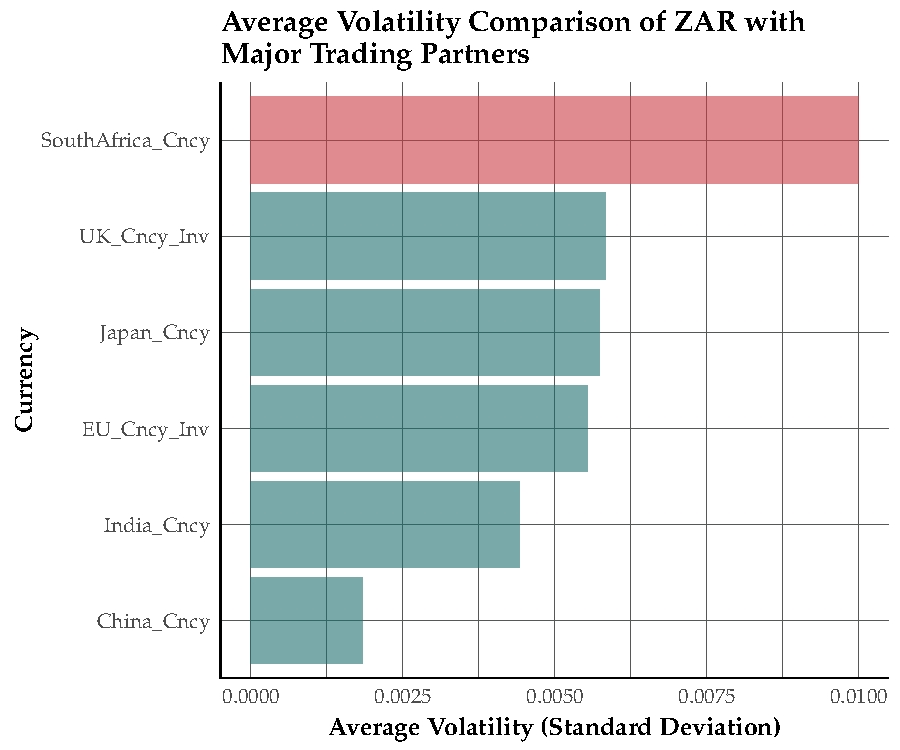
\includegraphics{Question-5_files/figure-latex/barplot-1.pdf}

Compared to major trading partners, the Rand on average has seen much
higher volatility over the past decade after the Global Financial Crisis
(GFC) of 2008, exhibiting average volatility (standard deviation) of
0.01 - almost double the volatility faced by trading partner currencies.

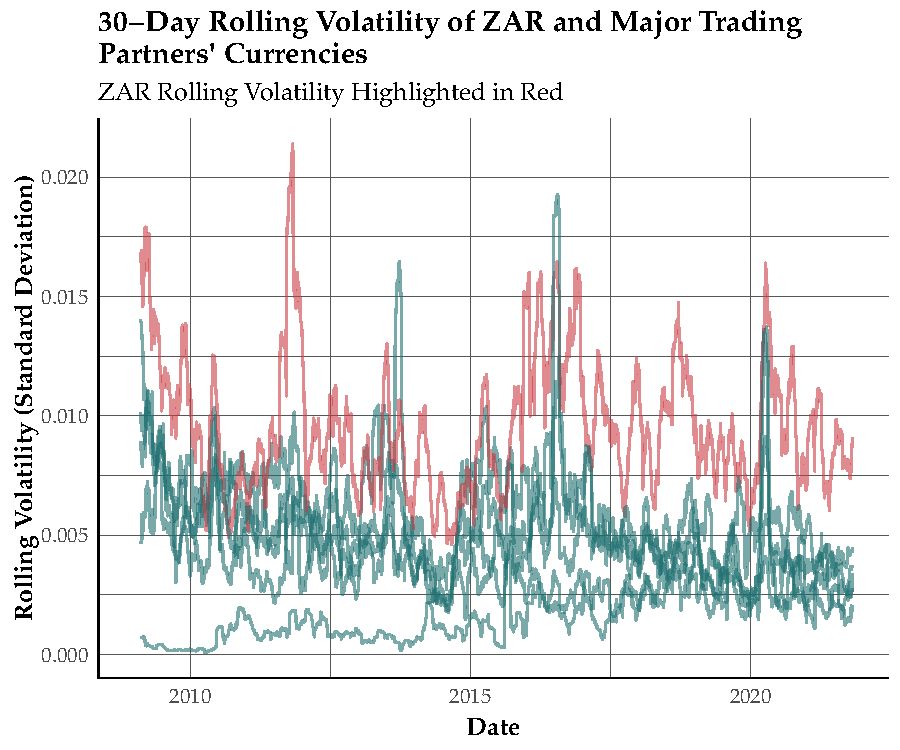
\includegraphics{Question-5_files/figure-latex/unnamed-chunk-1-1.pdf}

The ZAR consistently exhibited higher 30-day rolling volatility than
trading partners over the period under study. In the figure above, the
ZAR is highlighted in red.

Studying currency volatility involved fitting a GARCH(1,1) model to
estimate time-varying volatilities of multiple currencies, including the
South African Rand (ZAR). The model structure consisted of a GARCH(1,1)
framework. This model is designed to capture volatility clustering and
shocks in financial time series data. It works by modeling the
conditional variance of returns as a function of past squared returns
and past conditional variances. In simpler terms, it estimates how
volatile each currency's returns are at any given time, taking into
account its own historical volatility and squared returns, which helps
identify periods of high or low volatility. The model was applied
individually to each currency's returns, and the resulting conditional
volatilities were used for comparative analysis.

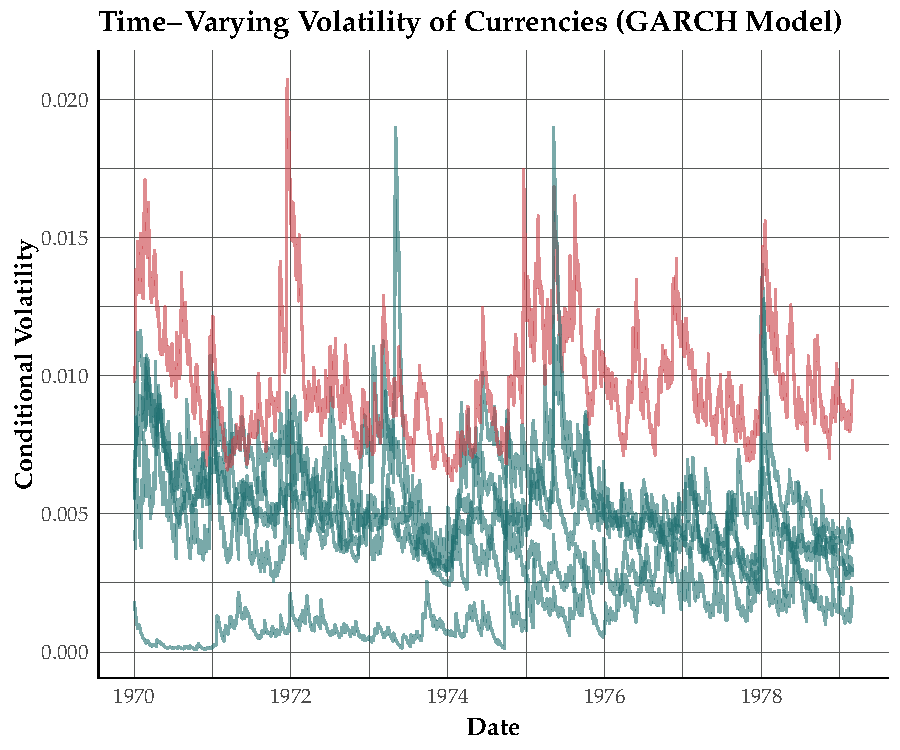
\includegraphics{Question-5_files/figure-latex/plot-garch-1.pdf}

The graph above indicates the South African Rand (ZAR) experiences
periods of higher volatility relative to its trading partners. These
peaks suggest moments of economic stress or significant market events.

A GO-GARCH model methodology was applied in the analysis and serves to
investigate the dynamic relationships between the South African Rand
(ZAR) and the currencies of the G10 countries. The GO-GARCH, or
Generalized Orthogonal GARCH, is a sophisticated variant of the standard
GARCH model which allows for the assessment of time-varying correlations
among multiple time series. In this context, the model captures how the
volatility of the ZAR co-moves with the volatility of the G10 currency
basket over time.

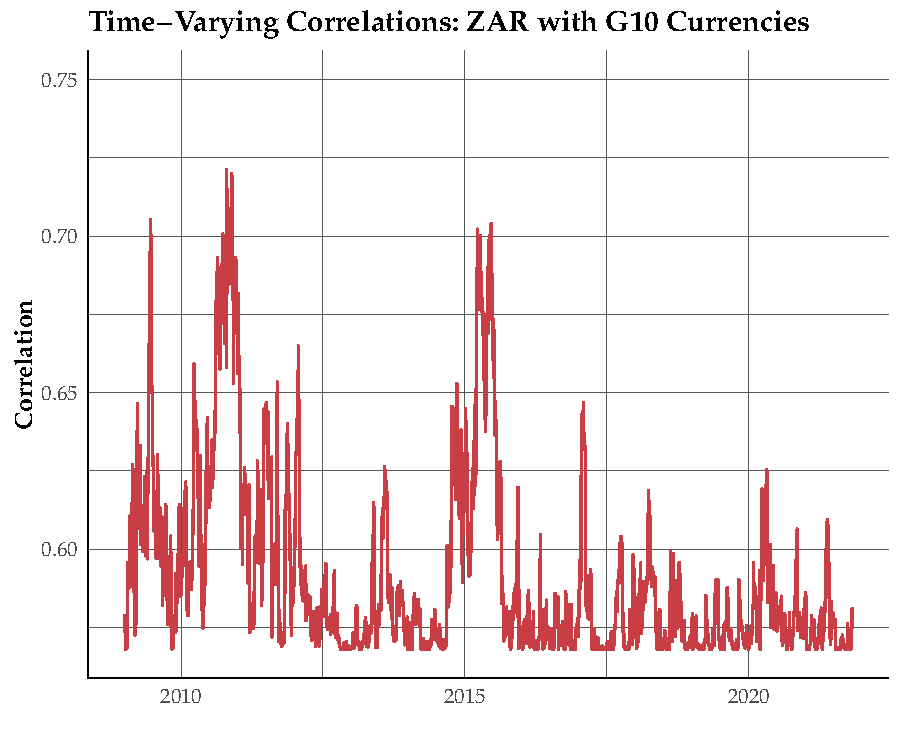
\includegraphics{Question-5_files/figure-latex/plot-gog-1.pdf}

The plot above illustrates the time-varying correlations between the
South African Rand (ZAR) and G10 currencies from 2010 to 2020. The
correlations fluctuate over time, displaying a range predominantly
between 0.55 and 0.75. Notably, there are peaks where the correlation
approaches 0.75, suggesting periods where the ZAR moved more in tandem
with the G10 currencies, possibly reflecting global economic events
impacting markets uniformly.

Conversely, the valleys indicate times when the ZAR had lower
correlations with the G10 currencies, which could imply periods where
local factors or idiosyncratic events had a greater impact on the ZAR's
movement, making it less aligned with the G10 currencies' trends.

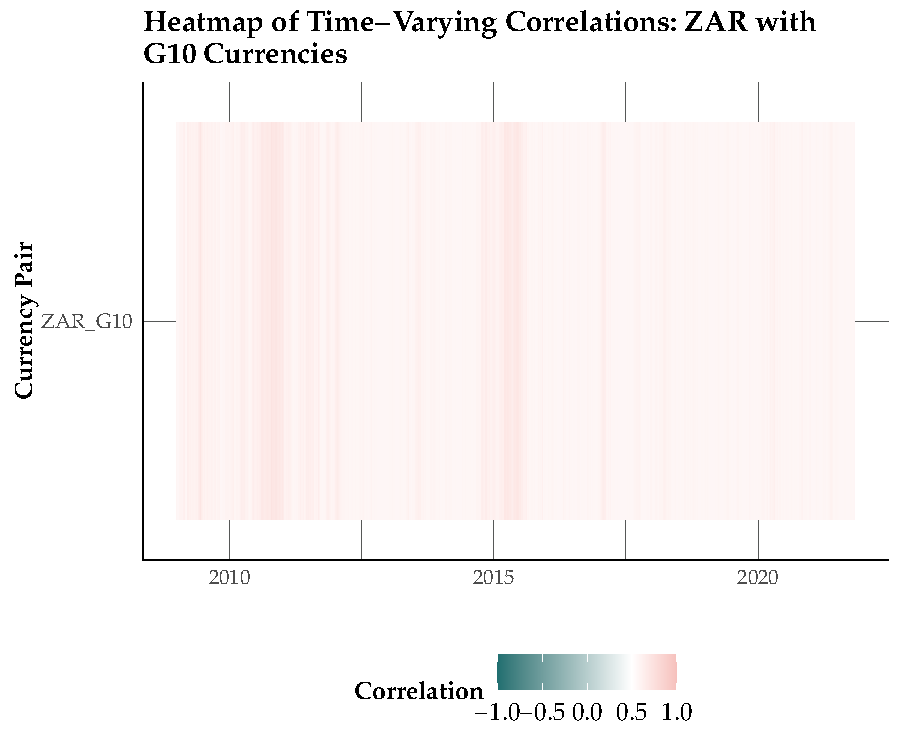
\includegraphics{Question-5_files/figure-latex/heat-map-1.pdf}

The heatmap depicts the time-varying correlations between the South
African Rand (ZAR) and G10 currencies from 2010 to around 2020. The
color gradient represents the strength of the correlation, where shades
closer to white denote a correlation near zero (indicating no
relationship), and darker shades, either red or blue, indicate stronger
positive or negative correlations respectively.

In this heatmap, however, the color gradient seems to be on a scale from
light to dark pink, suggesting that the correlations are predominantly
positive throughout the period. The intensity of the pink shade varies
over time, implying fluctuations in the degree of correlation. The
consistent presence of color, without reverting to white, indicates that
the ZAR generally maintains some level of positive correlation with the
G10 currencies during the given timeframe.

There aren't any dark red or blue patches, which would suggest extremely
high or low correlations, and the lack of variability in color intensity
indicates that while correlations fluctuate, they do so within a
relatively narrow range. This pattern might suggest that while specific
events or periods might affect the degree of co-movement between the ZAR
and G10 currencies, the overall relationship remains relatively stable
and positively correlated.

\bibliography{Tex/ref}





\end{document}
